% !TeX program = lualatex

% setup
\documentclass[
hyperref={bookmarks=false},
xcolor={dvipsnames,svgnames*,x11names*}, 
12pt
]{beamer}
\usepackage{../beamertheme/beamerinnerthemetb}
\usepackage{../beamertheme/beamerouterthemetb}
\usepackage{../beamertheme/beamercolorthemetb}
\usepackage{../beamertheme/beamerthemetb}

% packages
\usepackage{emoji}
\usepackage{graphicx}
\usepackage{xurl}
\usepackage{listings}

\lstset{
	basicstyle=\color{white}\ttfamily\scriptsize,
    backgroundcolor=\color{black}, 
    breaklines=true, 
    frame=single, 
    keepspaces=true, 
    escapechar={|},
    breakindent=0pt, 
    linewidth=1.025\linewidth
}

% options
\setlength{\leftmargini}{0cm}
\hypersetup{
	pdfauthor={Andrea Gilardi},
	colorlinks=true,
	urlcolor=Blue
}

%%% Define new stuff for slide numbers
\setbeamertemplate{navigation symbols}{}

\pgfkeys{/visual counter/.cd,
	thickness/.store in=\thickness,
	thickness=0.4ex,
	radius/.store in=\radius,
	radius=1.5ex,
	segment distance/.store in=\segdist,
	segment distance=8,
	color current frame/.store in=\colcurrframe,
	color current frame=orange,
	color old frame/.store in=\cololdframe,
	color old frame=blue,
	color next frame/.store in=\colnextframe,
	color next frame=gray!30,
	color page number/.store in=\colpagenum,
	color page number=white,
	current value/.store in=\currentv,
	current value=1,
	total value/.store in=\totalv,
	total value=2,
	circled page number/.code={
		\begin{tikzpicture}[fill color/.style={}]
			\pgfkeys{/visual counter/.cd, 
				current value=\insertframenumber,
				total value=\inserttotalframenumber,
			}
			\pgfmathtruncatemacro\current{\currentv+1}
			\def\tot{\totalv}
			\def\radiusout{\radius}
			\def\radiusin{\radius-\thickness}
			
			\foreach \s in {1,...,\tot}
			{
				\ifnum\s>\current%
				\tikzset{fill color/.append style={\colnextframe}}%
				\fi%
				\ifnum\s=\current%
				\tikzset{fill color/.append style={\colcurrframe}}%
				\fi%
				\ifnum\s<\current%
				\tikzset{fill color/.append style={\cololdframe}}%
				\fi%
				\fill[fill color]
				({90-360/\tot * (\s - 1)-\segdist}:\radiusout) arc 
				({90-360/\tot * (\s - 1)-\segdist}:{90-360/\tot * (\s)+\segdist}:\radiusout) --
				({90-360/\tot * (\s)+\segdist}:\radiusin) arc 
				({90-360/\tot * (\s)+\segdist}:{90-360/\tot * (\s - 1)-\segdist}:\radiusin);
				% new addition
				\node[inner sep=0pt,text=\colpagenum] at (0,0){\insertframenumber};
			}
		\end{tikzpicture}
	},
}

\setbeamertemplate{footline}{
	\begin{beamercolorbox}[wd=0.95\textwidth, ht=2ex,dp=1ex,sep=1ex]{footline}
		\hfill%
		\tikz\node[/visual counter/.cd,
		segment distance=-2pt,
		radius=0.33cm, thickness=0.33cm,
		color old frame=black,
		color current frame=black!80!gray!50,
		color next frame=black!80!gray!50,
		circled page number,
		]{};
	\end{beamercolorbox}
}
%%% End stuff for slide numbers

% metadata
\title{R4DS - Unit 3: Git \& Github or: How I Learned to Stop Worrying and Love Version Control\vspace{-1.25cm}}
\author{Andrea Gilardi}
\date{\today}

\begin{document}
\inserttitlepage

\begin{frame}{Outline and main concepts}
\vspace{-0.5cm}
\begin{itemize}
	\itemsep 3ex
	\item The objective of this unit is to introduce a Version Control System (VCS) named Git and its basic functionalities. 
	\item After installing the software, we will explore a simple but powerful workflow considering a local repository. Then, we will connect our PC to a remote repository on Github. 
	\item Finally, I will show you how to replicate (most of) the same steps using the Rstudio IDE. 
\end{itemize}
\end{frame}

\begin{frame}{About Version Control}
\vspace{-0.5cm}
\begin{itemize}
\itemsep 3ex
\item Version control is a system that records changes to a set of files over time so that you can recall specific versions later.
\item For example, if you are developing an algorithm for a new statistical procedure, Version Control Systems (VCS) allow you to revert files back to a previous state in case of bugs. 
\item You can also compare files over times, see which changes introduced the bug and revert back to a working state. 
\item \textbf{If you screw up, you can ``easily" recover!}. 
\end{itemize}
\end{frame}

\begin{frame}{What is Git?}
\vspace{-0.5cm}
\begin{itemize}
	\itemsep 3ex
	\item Git\footnote{Why is it named like that? See the last paragraph \href{https://github.com/git/git\#readme}{here}!} is a Distributed VCS, which means that you always have the entire history of the project at your disposal.
	\item It is a particularly efficient tool for large projects and it has a branching system that allows for non-linear development. 
	% \item As we will see, Git has three main states that your files can reside in: \textbf{modified}, \textbf{staged}, and \textbf{committed}. What does it mean? 
	
	\item At the beginning, we will work with the Git Shell. Then, I will show you how to integrate Git and Rstudio. 
\end{itemize}
\end{frame}

\setlength{\leftmarginii}{-1cm}

\begin{frame}{Install git}
\vspace{-0.5cm}

First, you need to check if you've already installed git! Run the following from your shell: \texttt{git --version}. \\
\vspace{1em}
If you see \texttt{git command not found}, keep reading! 

\begin{description}
\item[Windows: ] Download installer from \href{https://git-scm.com/download/win}{here}. A few notes: 
\begin{itemize}
\item You should install git under \texttt{C:/Program Files}.
\item When asked about \texttt{Adjusting your PATH environment}, make sure to select \texttt{Git from the command line and also from 3rd-party software}. 
\end{itemize}
\hspace{-1cm}Let's do it together! 
\item[macOS: ] The shell should prompt you to install it after running the previous command. See also \href{https://git-scm.com/download/mac}{here}. 
\end{description}
\end{frame}

\setlength{\leftmarginii}{-1.5cm}

\begin{frame}{First time git setup}
\vspace{-0.5cm}
First, we can slightly customize the Git environment. 
\begin{description}
\item[Setup identity:] Run the following commands
\begin{itemize}
\item \texttt{git config --global user.name "Andrea Gilardi"}
\item \texttt{git config --global user.email andrea.gilardi@unimib.it}
\end{itemize}
\hspace{-2cm} Please use the same email as the github account.
\item[Setup editor:] See \href{https://git-scm.com/book/en/v2/Appendix-C\%3A-Git-Commands-Setup-and-Config\#ch_core_editor}{here} for instructions. 
\item[Default branch name:] You can run 
\begin{itemize}
\item \texttt{git config --global init.defaultBranch main}
\end{itemize}  
\hspace{-2cm} The default name for the initial branch is \texttt{master}. 
\item[Check settings:] Run \texttt{git config --list}
\end{description}
\end{frame}

\begin{frame}{Git Basics\emoji{grinning-face-with-sweat}...}
\vspace{-0.5cm}
\begin{figure}
\centering
\includegraphics[width=0.85\linewidth]{figures/incaseoffire.pdf}
\end{figure}
\href{https://hikaruzone.wordpress.com/2015/10/06/in-case-of-fire-1-git-commit-2-git-push-3-leave-building/}{\textbf{Source}}. Don't worry, now we are going to review many many more details! 
\end{frame}

\setlength{\leftmarginii}{0.25cm}

\begin{frame}{My first Git repo!}
\vspace{-0.5cm}
We can create a Git repository in two ways: 
\begin{enumerate}
\itemsep 2ex	
\item Take a local directory and initialise a Git structure.
\begin{itemize}
\item Create an empty directory where you will store your files;  
\item Open the shell inside the new repo and run \texttt{git init}. 
\end{itemize}
\item Clone an existing repository stored online. 
\begin{itemize}
\item Open the shell into the parent repository; 
\item Run \texttt{git clone <url>}. For example, run \texttt{git clone https://github.com/agila5/R4DS-PhD-Unimib.git}. 
\end{itemize}
\end{enumerate}
At the end of the class, we will see how to create a Git repo on Github and clone it on your local computer. 
\end{frame}

\begin{frame}{Git basics - A graphical abstract}
	\vspace{-0.5cm}
	The following figure nicely summarises the algorithm used by Git to record changes in a repository. 
	\begin{figure}
		\centering
		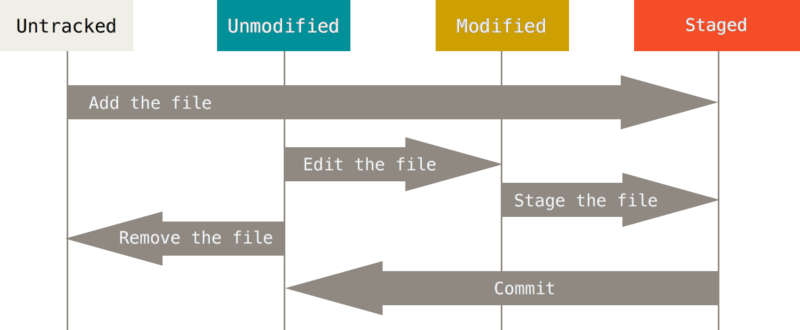
\includegraphics[width=\linewidth]{figures/lifecycle.png}
	\end{figure}
	\textbf{Source:} \url{https://git-scm.com/book/en/v2/Git-Basics-Recording-Changes-to-the-Repository}
\end{frame}

\begin{frame}[fragile]{Git Status}
\vspace{-0.5cm}
\begin{itemize}
\itemsep 2ex
\item Let's create a local Git repo (e.g. \texttt{myFirstGitRepo})!
\item Open a (Git) shell inside the repo and run \texttt{git status}. You should see the following output: 

\begin{lstlisting}
On branch main

No commits yet

nothing to commit (create/copy files and use "git add" to track)
\end{lstlisting}

\item Now we need to create a new file (say \texttt{README.md}) and add some content (e.g. \texttt{"Hello World :)"}). 
\end{itemize}
\end{frame}

\begin{frame}[fragile]{Git Status (cont)}
\vspace{-0.5cm}
\begin{itemize}
\itemsep 2ex
\item Now you should see 
\begin{lstlisting}
On branch main
	
No commits yet
	
Untracked files:
(use "git add <file>..." to include in what will be committed)
     |\textcolor{red}{README.md}|
	
nothing added to commit but untracked files present (use "git add" to track)
\end{lstlisting}
\item Untracked basically means that Git sees a file you didn’t have in the previous snapshot, and which hasn’t yet been staged. Let's start tracking the file!
\end{itemize}
\end{frame}

\begin{frame}[fragile]{Tracking New Files}
\vspace{-0.5cm}
\begin{itemize}
\itemsep 2ex
\item We can run \texttt{git add README.md} to start tracking the new file. Then, if we run \texttt{git status} again we see
\begin{lstlisting}
On branch main

No commits yet

Changes to be committed:
  (use "git rm --cached <file>..." to unstage)
       |\textcolor{green}{new file:   README.md}|
\end{lstlisting}
\item Now \texttt{README.md} file is staged\footnote{Staged means ``ready to go into the next commit snapshot".} and we can commit\footnote{Committed means ``saved in the local database".} by running \texttt{git commit -m "Some text"}.  
\end{itemize}
\end{frame}

\begin{frame}[fragile]{Committing Your Changes}
\vspace{-0.5cm}
\begin{itemize}
\itemsep 2ex
\item You should see something like
\begin{lstlisting}
$ git commit  -m "first commit - add README.md"
[main (root-commit) 3b94fbf] first commit - add README.md
1 file changed, 1 insertion(+)
create mode 100644 README.md
\end{lstlisting}
We can see that the message describes some details about the commit (the branch, how many files were changed \dots)
\item If we check the status again\dots
\begin{lstlisting}
$ git status
On branch main
nothing to commit, working tree clean	
\end{lstlisting}
\end{itemize}
\end{frame}

\begin{frame}[fragile]{Let's do it again!}
\vspace{-0.5cm}
\begin{itemize}
\itemsep 2ex
\item Let's create a new file (say \texttt{CONTRIBUTING.md}) and add some text to it. Now, if we ran \texttt{git status}, we would see the same output as before (just with a different file name). 
\item Let's modify also \texttt{README.md} adding some text. Now we see
\begin{lstlisting}
[truncated...]
Changes not staged for commit:
(use "git add <file>..." to update what will be committed)
(use "git restore <file>..." to discard changes in working directory)
      |\textcolor{red}{modified:   README.md}|

Untracked files:
(use "git add <file>..." to include in what will be committed)
      |\textcolor{red}{CONTRIBUTING.md}|

[truncated...]
\end{lstlisting}
\end{itemize}
\end{frame}

\begin{frame}[fragile]{Let's do it again! (cont)}
\vspace{-0.5cm}
\begin{itemize}
\itemsep 2ex
\item The output says that the \textbf{tracked} file \texttt{README.md} has been modified in the directory but is not \textbf{staged} yet. We can stage both files running \texttt{git add .} and now we see
\begin{lstlisting}
$ git status
On branch main
Changes to be committed:
(use "git restore --staged <file>..." to unstage)
      |\textcolor{green}{new file:   CONTRIBUTING.md}|
      |\textcolor{green}{modified:   README.md}|
\end{lstlisting}

\item Now we could run \texttt{git commit -m "\dots"} as before. But what happens if we modified a staged file? Let's add even more text to \texttt{README.md}. 
\end{itemize}
\end{frame}

\begin{frame}[fragile]{Let's do it again! (cont)}
\vspace{-0.5cm}
\begin{itemize}
\itemsep 2ex
\item We see the following
\begin{lstlisting}
$ git status
On branch main
Changes to be committed:
(use "git restore --staged <file>..." to unstage)
      |\textcolor{green}{new file:   CONTRIBUTING.md}|
      |\textcolor{green}{modified:   README.md}|

Changes not staged for commit:
(use "git add <file>..." to update what will be committed)
(use "git restore <file>..." to discard changes in working directory)
      |\textcolor{red}{modified:   README.md}|
\end{lstlisting}
\item If you commit now, you will preserve the currently staged version of \texttt{README.md}. You can run \texttt{git add README.md} again in case you need to update the file version. 
\end{itemize}
\end{frame}

\begin{frame}[fragile]{Let's do it again! (cont)}
\vspace{-0.5cm}
\begin{itemize}
\itemsep 2ex
\item The \texttt{git diff} command can be used to see what we changed but not yet staged: 
\begin{lstlisting}
$ git diff
diff --git a/README.md b/README.md
index dd577f0..3d6d21b 100644
--- a/README.md
+++ b/README.md
|\textcolor{blue}{@@ -1,2 +1,3 @@}|
Hallo World :)
|\textcolor{red}{-Hallo World 2 :)}|
\ No newline at end of file
|\textcolor{green}{+Hallo World 2 :)}|
|\textcolor{green}{+Hallo World 3 :)}|
\ No newline at end of file
\end{lstlisting}
\item And if we want to compare the currently staged file with the previous commit? Then, use \texttt{git diff --staged}. 
\end{itemize}
\end{frame}

\begin{frame}[fragile]{Let's do it again! (cont)}
\vspace{-0.5cm}
\begin{itemize}
\itemsep 2ex
\item Now you should see
\begin{lstlisting}
$ git diff --staged
diff --git a/CONTRIBUTING.md b/CONTRIBUTING.md
new file mode 100644
index 0000000..b3da348
--- /dev/null
+++ b/CONTRIBUTING.md
|\textcolor{blue}{@@ -0,0 +1 @@}|
|\textcolor{green}{+You are welcome to contribute to my repo :)}|
\ No newline at end of file
diff --git a/README.md b/README.md
index bf231b1..dd577f0 100644
--- a/README.md
+++ b/README.md
|\textcolor{blue}{@@ -1 +1,2 @@}|
|\textcolor{red}{-Hallo World :)}|
\ No newline at end of file
|\textcolor{green}{+Hallo World :)}|
|\textcolor{green}{+Hallo World 2 :)}|
\ No newline at end of file
\end{lstlisting}
\end{itemize}
\end{frame}

\begin{frame}[fragile]{Let's do it again! (cont)}
\vspace{-0.5cm}
\begin{itemize}
\itemsep 2ex
\item Now, after staging all files and committing, we should see 
\begin{lstlisting}
$ git status
On branch main
nothing to commit, working tree clean
\end{lstlisting}
\item \textbf{NB:} If you add the \texttt{-a} flag to \texttt{git commit}, then Git automatically stage every file \textbf{that is already tracked} before doing the commit. 
\end{itemize}
\end{frame}

\begin{frame}[fragile]{Ignoring files}
\vspace{-0.5cm}
\begin{itemize}
\itemsep 2ex
\item A \texttt{.gitignore} file can be used to tell Git not to track certain types of files (e.g. log files). 
\item Let's create a \texttt{example.log} file inside our repo. We see 
\begin{lstlisting}
$ git status
On branch main
Untracked files:
(use "git add <file>..." to include in what will be committed)
      |\textcolor{red}{example.log}|

nothing added to commit but untracked files present (use "git add" to track)
\end{lstlisting}
\end{itemize}
\end{frame}

\begin{frame}[fragile]{Ignoring files (cont)}
\vspace{-0.5cm}
\begin{itemize}
\itemsep 2ex
\item If we create a \texttt{.gitignore} file that includes the path of the new file (i.e. \texttt{example.log}), then we see
\begin{lstlisting}
$ git status
On branch main
Untracked files:
(use "git add <file>..." to include in what will be committed)
      |\textcolor{red}{.gitignore}|

nothing added to commit but untracked files present (use "git add" to track)
\end{lstlisting}
\item More details: \url{https://git-scm.com/book/en/v2/Git-Basics-Recording-Changes-to-the-Repository}
\end{itemize}
\end{frame}

\begin{frame}[fragile]{I f*ucked up \emoji{loudly-crying-face} \texttt{--amend}!}
\vspace{-0.5cm}
\begin{itemize}
\itemsep 2ex
\item The \texttt{--amend} option can be used to rectify a \texttt{git commit} message. For example, if we run
\begin{lstlisting}
$ git add . 
$ git commit -m "a typo here :("
\end{lstlisting} 
then we can adjust the text with
\begin{lstlisting}
$ git commit --amend -m "the right text now!"
\end{lstlisting}
\item Check the commit history with \texttt{git log}!
\item The \texttt{--amend} option works analogously if we add more files to the staged area. 
\end{itemize}
\end{frame}

\begin{frame}[fragile]{I f*ucked up \emoji{loudly-crying-face} \texttt{git restore}!}
\vspace{-0.5cm}
\begin{itemize}
\itemsep 2ex
\item As we saw from the previous messages, \texttt{git restore --staged <file>} can be used to unstage a file. We can test it by modifying the \texttt{.gitignore file} explicitly forcing Git to ignore \texttt{.Rdata} files (see Unit 1!).
\item Similarly, \texttt{git restore <file>} can be used to discard unstaged changes so that a file looks like when we last committed it! Let's remove the \texttt{.Rdata} string from \texttt{.gitignore}. 
\end{itemize}
\end{frame}

\begin{frame}{Other commands}
\vspace{-0.5cm}
As you can imagine, there are several more useful Git commands but we are not going to review all of them. A (not-comprehensive) list: 
\begin{itemize}
\itemsep 2ex
\item \texttt{git rm}: remove a file from Git (see also previous messages); 
\item \texttt{git mv}: record a file movement; 
\item \texttt{git log}: explore the commits' history.
\end{itemize}
During the next units, we will explore \texttt{git blame} and \texttt{git bisect} (which are useful for debugging Git projects). 
\end{frame}

\begin{frame}{Github!}
\vspace{-0.5cm}
\begin{itemize}
\itemsep 2ex
\item \textbf{Github} is an hosting service that provides home for Git-based projects. Github allows other people to see your work, but it is a also good idea to save your (solo) projects on Github (as a backup in case you screw up badly). 
\item The first thing to do is to create an account. \href{https://github.com/signup?ref_cta=Sign+up\&ref_loc=header+logged+out\&ref_page=\%2F\&source=header-home}{Signup}. 
\item See \href{https://happygitwithr.com/github-acct.html}{here} if you need a few suggestions for choosing your github name. See also \href{https://happygitwithr.com/big-picture.html}{this} Chapter (and the whole book) for a more complete description of Git/Github.  
\item Now we need to complete the most difficult step: synch (local) Git with (remote) Github\dots
\end{itemize}
\end{frame}

\begin{frame}{Can you hear me now?}
\vspace{-0.5cm}
\begin{itemize}
\itemsep 2ex
\item When you interact with a remote Git server, you need to include your credentials into the request (otherwise everybody can add files to your repo, which is bad\dots). 
\item Git can adopt two different protocols: HTTPS and SSH. Here we focus on HTTPS. Check the references of this course if you want to explore the other protocol. 
\item An HTTPS protocol uses a Personal Access Token (PAT) to add private credentials into your request. 
\end{itemize}
\end{frame}

\begin{frame}[fragile]{Can you hear me now? (cont)}
\vspace{-0.5cm}
\begin{itemize}
\itemsep 2ex
\item For us, the easiest way to generate a PAT is running the following R commands: 
\begin{lstlisting}[basicstyle=\color{black}\ttfamily\scriptsize, backgroundcolor=\color{white}]
install.packages(c(|\textcolor{ForestGreen}{"usethis"}|, |\textcolor{ForestGreen}{"gitcreds"}|))
usethis::create_github_token()
\end{lstlisting}
\item Then, store the PAT explicitly by running
\begin{lstlisting}[basicstyle=\color{black}\ttfamily\scriptsize, backgroundcolor=\color{white}]
gitcreds::gitcreds_set()
\end{lstlisting} 
to get a prompt where you can paste your PAT. 
\item See \href{https://happygitwithr.com/https-pat.html}{here} for many more details and troubleshooting. 
\item Now we can finally \href{https://github.com/new}{create} our first Github repo and clone it.
\end{itemize}
\end{frame}

\begin{frame}{Git and Github}
\vspace{-0.5cm}
Now  let's recap the whole process: 
\begin{enumerate}
\itemsep 2ex
\item Create an (empty) repository on Github; 
\item Clone the repository on your computer (i.e. \texttt{git clone});
\item Add a \texttt{README.md} file with some content; 
\item Stage the new file and create a new commit; 
\item Push the new commit on Github (i.e. \texttt{git push}); 
\item Check the result and celebrate \emoji{partying-face}  
\end{enumerate}
\end{frame}

\begin{frame}{Git, Github and Rstudio}
\vspace{-0.5cm}
Now, let's delete the Git repo (after pushing the new commit) and repeat the same process from Rstudio. 
\begin{enumerate}
\itemsep 2ex
\item Open Rstudio and Click on "Create a Project"; 
\item Select Version Control -> Git and copy the URL from github. Then click on Create Project. 
\end{enumerate}
The output is a Git folder with the same file as before but it includes also an Rstudio project. Finally, 
\begin{enumerate}
\item explore the new (automatically-defined) \texttt{.gitignore} file;
\item create a new \texttt{.R} file and commit with the Git control panel.
\end{enumerate}
\end{frame}

\begin{frame}[fragile]{More details on remotes}
\vspace{-0.5cm}
\begin{itemize}
\itemsep 2ex
\item As you can imagine, there is nothing special with Github and we can use a similar process to connect a local Git repo with other hosting service (e.g. Gitlab) and other remotes.  
\item The command \texttt{git remote} can list the remotes: 
\begin{lstlisting}
$ git remote -v
origin  https://github.com/agila5/R4DS-PhD-Unimib.git (fetch)
origin  https://github.com/agila5/R4DS-PhD-Unimib.git (push)
\end{lstlisting}
\item See \url{https://git-scm.com/book/en/v2/Git-Basics-Working-with-Remotes} for more details. We will also re-examine this topic when we talk about branches. 
\end{itemize}
\end{frame}

\newcounter{myenumi}

\begin{frame}{Homework!}
\vspace{-0.5cm}
\begin{enumerate}
\itemsep 1ex
\item Create an (empty) repository on Github named \texttt{GithubHomework}; 
\item Clone it on your computer using the Rstudio IDE; 
\item Create a \texttt{README.md} file that contains a minimal description of the repository. Push the new file on Github including an informative commit message and check the output locally and online. \textbf{NB:} Run \texttt{git status} frequently.  
\item Add a new directory named \texttt{R} and, into the new directory, create two new files named \texttt{GithubHomework.log} and \texttt{script.R}, respectively. 
\item Ignore the \texttt{.log} file and commit the \texttt{.R} file using the following message: \texttt{"BLABLABLA"}. Double check it to be 100\% sure. 
\setcounter{myenumi}{\value{enumi}}
\end{enumerate}
\end{frame}

\begin{frame}{Homework! (cont)}
\vspace{-0.5cm}
\begin{enumerate}
\setcounter{enumi}{\value{myenumi}}
\item Amend the previous commit message adopting a more informative one. 
\item Push the new changes to the remote (i.e. Github). 
\item How can you modify the message for a commit that you've already pushed? \textbf{Google is your friend} \emoji{smile}. 
\item Check that you completed the previous task by exploring the history of the project both from Git (i.e. \texttt{git log}) and from Github (again, ask to Google!). 
\end{enumerate}
\end{frame}
\end{document}